\section{Introduction}

\subsection{Problème de Stigler}

	$x_i$ est la quantité du i\ieme{} aliment ($i = 1,\dots,77$).
	Le problème de Stigler s'écrit comme suit:
	\begin{equation*}
	\renewcommand{\arraystretch}{1.5}
	\begin{array}{c@{\quad} l c r@{\quad} l}
		\min\limits_{\bm{x}} & \sum\limits_{i = 1}^{77} c_i x_i & & & \\
		\textnormal{s.t.} & \sum\limits_{i = 1}^{77} A_{ij} x_i & \ge & b_j\,, & \forall j\,,\\
		& \multicolumn{1}{r}{x_i} & \ge & 0\,, & \forall i\,,
	\end{array}
	\end{equation*}
	où
	\begin{itemize}
		\item $c_i$ est le coût par unité de poids de $i$,
		\item $b_j$ est la quantité cible du nutriment $j$,
		\item $A_{ij}$ est la quantité du nutriment $j$
		dans l'aliment $i$ (par unité de poids).
		On a donc $A \in \R^{9 \times 77}$.
	\end{itemize}

	Notons que la première contrainte
	peut se réécrire en notation matricielle comme
	(par la suite,
	on omettra les notations spéciales pour les vecteurs et matrices):
	\[
	Ax \ge b\,.
	\]
	Dans cette équation,
	le signe ``$\ge$'' désigne
	l'\emph{element-wise greater than or equal to}
	(plus grand ou égal élément par élément).

	Notons également que ``s.t.'' est l'abbréviation de ``subject to''.

\subsection{Problème en deux dimensions}

	Montrons maintenant une façon graphique
	de résoudre un problème d'optimisation linéaire.
	Évidemment, cette méthode n'est \textit{a priori} utile
	que pour les problèmes en deux dimensions.

	Soit le problème suivant:
	\begin{equation*}
	\begin{array}{c@{\quad} r c r c r@{\quad} l}
		\max\limits_{x} & x_1 & + & 2 x_2 & & &\\
		\textnormal{s.t.} & & & x_2 & \le & 6 &\\
		& x_1 & & & \le & 8 &\\
		& 3 x_1 & + & 4 x_2 & \le & 36 & \\
		& & & x_i & \ge & 0 & \forall i\,.
	\end{array}
	\end{equation*}

	Graphiquement, on obtient la figure suivante:

	\begin{center}
	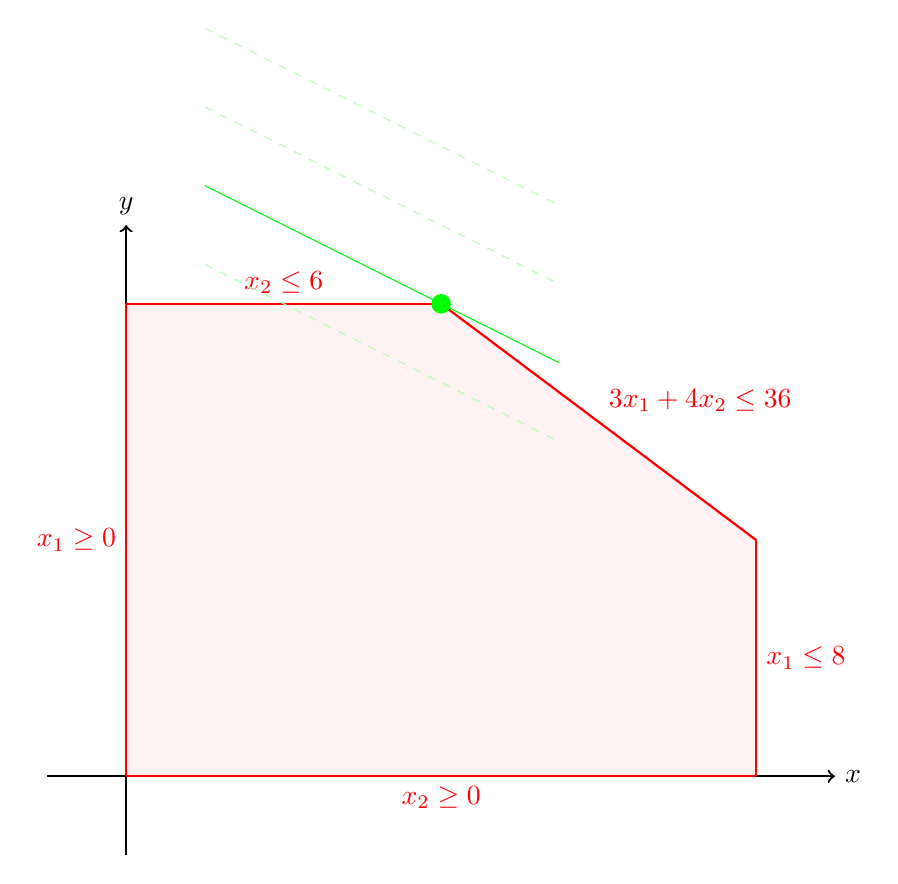
\begin{tikzpicture}
		\draw[->,thick] (-1,0)--(9,0) node[right]{$x$};
		\draw[->,thick] (0,-1)--(0,7) node[above]{$y$};

		\coordinate (O) at (0,0);
		\coordinate (A) at (0,6);
		\coordinate (B) at (4,6);
		\coordinate (C) at (8,3);
		\coordinate (D) at (8,0);

		\draw[fill=red!5] (O) -- (A) -- (B) -- (C) -- (D) -- cycle;

		\draw[color=red,thick] (O) -- (A) node[midway, left] {$x_1 \ge 0$};
		\draw[color=red,thick] (A) -- (B) node[midway, above] {$x_2 \le 6$};
		\draw[color=red,thick] (B) -- (C) node[midway, above right] {$3x_1 + 4 x_2 \le 36$};
		\draw[color=red,thick] (C) -- (D) node[midway, right] {$x_1 \le 8$};
		\draw[color=red,thick] (O) -- (D) node[midway, below] {$x_2 \ge 0$};

		\draw [dashed, domain=1:5.5,samples=200, color=green!30] plot(\x,{10 - 0.5*\x});
		\draw [dashed, domain=1:5.5,samples=200, color=green!30] plot(\x,{9 - 0.5*\x});
		\draw [domain=1:5.5,samples=200, color=green] plot(\x,{8 - 0.5*\x});
		\draw [dashed, domain=1:5.5,samples=200, color=green!30] plot(\x,{7 - 0.5*\x});

		\node at (B) [circle,fill=green,inner sep=2.5pt] {};

	\end{tikzpicture}
	\end{center}

	Le point vert est appelé la solution optimale,
	alors que la surface rouge est appelée
	l'ensemble des solutions admissibles.

	Pour voir que le point vert est optimal,
	il suffit de proposer à la suite plusieurs valeurs optimales,
	jusqu'à se rendre compte qu'à chaque valeur optimale correspond
	une fonction objectif.
	On voit que le premier point de l'ensemble admissible atteint ainsi
	est bien le point vert.

\subsection{Problème de flots (ou de transport)}

	\begin{center}
	\begin{tikzpicture}
		\node [rectangle] (cij) at (-3,-3) {$c_{ij}$};
		\node [rectangle] (bitop) at (-3,0) {$b_{i}$};
		\node [rectangle] (bibottom) at (-3,-6) {$b_{i}$};

		\begin{scope}[every node/.style={circle,thick,draw,minimum size=1cm}]
			\node (P1) at (0,0) {$+10$};
			\node (P2) at (3,0) {$+5$};
			\node (P3) at (6,0) {$+10$};
			\node (C1) at (0,-6) {$-12$};
			\node (C2) at (3,-6) {$-5$};
			\node (C3) at (6,-6) {$-8$};

		\begin{scope}[>={Stealth[black]}, every node/.style={fill=white,circle}, every edge/.style={draw=red,very thick}]
			\path [->] (P1) edge[bend right=10] node {$5$} (C1);
			\path [->] (P1) edge node {$3$} (C2);
			\path [->] (P1) edge[bend left=16] node {$2$} (C3);
			\path [->] (P2) edge[bend right=18] node {$4$} (C1);
			\path [->] (P2) edge node {$7$} (C2);
			\path [->] (P3) edge[bend left=16] node {$\frac{1}{2}$} (C1);
			\path [->] (P3) edge node {$3$} (C2);
			\path [->] (P3) edge[bend left=20] node {$4$} (C2);
			\path [->] (P3) edge node {$1$} (C3);
		\end{scope}
		\end{scope}
	\end{tikzpicture}
	\end{center}

	Par convention, les arêtes non dessinées ont un coût infini.

	Le problème s'écrit sous forme mathématique comme suit:
	\begin{equation*}
	\begin{array}{c@{\quad} c c r c r@{\quad} l}
		\min\limits_{x} & \sum\limits_{{\displaystyle (i,j) \in \mathcal{E}}} c_{ij}x_{ij} &&&&& \\
		\textnormal{s.t.} & \sum\limits_{{\displaystyle j \suchthat (i,j) \in \mathcal{E}}} x_{ij} & - & \sum\limits_{{\displaystyle j \suchthat (j,i) \in \mathcal{E}}} x_{ji} & = & b_i\,, & \forall i\,,\\
		&&& x_{ij} & \ge & 0\,, & \forall i,j\,,
	\end{array}
	\end{equation*}
	où
	\begin{itemize}
		\item les $x_{ij}$ sont les quantités transportées de $i$ à $j$,
		\item les $c_{ij}$ sont les coûts unitaires de transport
		de $i$ à $j$,
		\item les $b_i$ sont les ``bilans'' des n\oe{}uds
		\item et $\mathcal{E}$ est l'ensemble des paires $(i,j)$.
	\end{itemize}

\subsection{Problème discret}

	Les problèmes discrets sont plus difficiles et plus coûteux
	au niveau du temps de calcul.
	Cela implique qu'on n'a plus le même problême que dans le cas continu.

\subsection{Problème d'affectation}
\label{sec:affectation}

	\begin{center}
	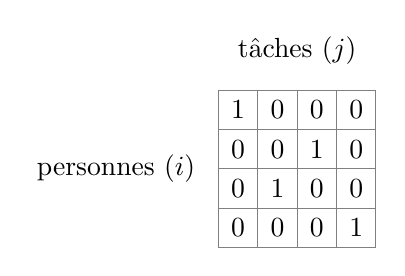
\begin{tikzpicture}
		\node [rectangle] (pers) at (-2.3,0) {personnes ($i$)};
		\node [rectangle] (taches) at (0,1.5) {tâches ($j$)};

		\draw[step=0.5cm,color=gray] (-1,-1) grid (1,1);
			\node at (-0.75,+0.75) {1};
			\node at (-0.25,+0.75) {0};
			\node at (+0.25,+0.75) {0};
			\node at (+0.75,+0.75) {0};
			\node at (-0.75,+0.25) {0};
			\node at (-0.25,+0.25) {0};
			\node at (+0.25,+0.25) {1};
			\node at (+0.75,+0.25) {0};
			\node at (-0.75,-0.25) {0};
			\node at (-0.25,-0.25) {1};
			\node at (+0.25,-0.25) {0};
			\node at (+0.75,-0.25) {0};
			\node at (-0.75,-0.75) {0};
			\node at (-0.25,-0.75) {0};
			\node at (+0.25,-0.75) {0};
			\node at (+0.75,-0.75) {1};
	\end{tikzpicture}
	\end{center}

	Le problème d'affectation revient à dire
	qu'on a un certain nombre de personnes
	qui peuvent chacune faire une parmi plusieurs tâches.
	La façon la plus efficace de représenter ce problème
	est à l'aide d'une matrice (appelée matrice d'affectation)
	qui dit si oui ou non une personne $i$
	fait la tâche $j\,$.
	Chaque tâche à un certain coût $p_i$ pour la personne $i\,$.
	Si la personne $i$ fait la tâche $j$, $x_{ij}$ vaut 1,
	sinon il vaut 0.
	Sous forme mathématique, on a
	\begin{equation*}
	\begin{array}{c@{\quad} r c l@{\quad} l}
		\min\limits_{x} & \sum\limits_{{\displaystyle (i,j) \in \mathcal{E}}} p_i x_{ij} &&&\\
		\textnormal{s.t.} & x_{ij} & \in & \{0, 1\}\,, & \forall i,j\,.
	\end{array}
	\end{equation*}
	où $\mathcal{E}$ est l'ensemble
	des paires (personne, tâche) possibles.
	Le problème d'affectation est donc \textit{a priori}
	un problème de flots discret.
